%                                                                 aa.dem
% AA vers. 9.1, LaTeX class for Astronomy & Astrophysics
% demonstration file
%                                                       (c) EDP Sciences
%-----------------------------------------------------------------------
%
%\documentclass[referee]{aa} % for a referee version
%\documentclass[onecolumn]{aa} % for a paper on 1 column  
%\documentclass[longauth]{aa} % for the long lists of affiliations 
%\documentclass[letter]{aa} % for the letters 
%\documentclass[bibyear]{aa} % if the references are not structured 
%                              according to the author-year natbib style


%
\documentclass{aa}  

%
\usepackage{graphicx}
%%%%%%%%%%%%%%%%%%%%%%%%%%%%%%%%%%%%%%%%
\usepackage{txfonts}
%%%%%%%%%%%%%%%%%%%%%%%%%%%%%%%%%%%%%%%%
\usepackage{amsmath}
\usepackage{mathrsfs}
\usepackage{booktabs}
\usepackage{hyperref}
%\usepackage[options]{hyperref}
% To add links in your PDF file, use the package "hyperref"
% with options according to your LaTeX or PDFLaTeX drivers.
%
\begin{document} 

   \title{Polytropic Stellar Model}
   
   \subtitle{Project II - Computational Astronomy}

   \author{Rui Peixoto}

   \institute{Departamento de Física e Astronomia, Faculdade de Ciências,
     Universidade do Porto}

%   \date{Received September 15, 1996; accepted March 16, 1997}

% \abstract{}{}{}{}{} 
% 5 {} token are mandatory
 
  \abstract
  % context heading (optional)
  % {} leave it empty if necessary  
   {}
  % aims heading (mandatory)
   {Stellar structure is studied by constructing a polytropic model for main
     sequence stars. A computational method for determining polytropic indexes
     from data is developed and implemented. Regime of application and possible
     improvements to the model are discussed.}
  % methods heading (mandatory)
   {Numerical solutions to the Lane-Emden equation are computed from given data
     (mass, radius and chemical properties) and luminosity boundary conditions
     are satisfied employing a shooting method. Uncertainty is modeled by
     repeated sampling (Monte Carlo).}
  % results heading (mandatory)
   {An efficient numerical method for simulating stellar structure
     in polytropic conditions is developed and applied to the study of the
     $\alpha$ Centauri AB binary.}
  % conclusions heading (optional), leave it empty if necessary 
   {}

   \maketitle
%
%-------------------------------------------------------------------

\section{Introduction}

As a major branch of astrophysics, the study of stars and their structure takes
an important role in the understanding of the origin and dynamics of the
Universe, at both local and cosmological scale, simultaneously
constituting a powerful tool in the context of nuclear and plasma physics.

For the most comprehensive description of stellar interiors, observational data
of multiple sources may be combined with theoretical models and numerical
simulations, motivating the following study.

Modeling these objects starts by considering hydrostatic equilibrium (equation
\ref{eq:hydrostatic_equilibrium}) and mass conservation (equation
\ref{eq:mass_conservation}), where $P$ is pressure, $\rho$ density, $\vec{v}$ velocity, and $\phi$
gravitational potential, following the Poisson equation, as well as spherical symmetry.

\begin{equation}
  \label{eq:hydrostatic_equilibrium}
  \rho \frac{\mathrm{d} \vec{v}}{\mathrm{d} t}=-\nabla P-\rho \nabla \phi
\end{equation}
\begin{equation}
  \label{eq:mass_conservation}
  \frac{\partial \rho}{\partial t}+\nabla \cdot(\rho \vec{v})=0
\end{equation}

For main sequence stars, one may assume a polytropic relation between the
temperature $T$ and pressure of the kind displayed in equation
\ref{eq:poly_relation}, for a real constant $K$.

\begin{equation}
  \label{eq:poly_relation}
  P=K \rho^{1+\frac{1}{n}}
\end{equation}

Combining these equation in terms of adimensional variables $\theta = \left(
  \frac{\rho}{\rho_c} \right)^\frac{1}{n}$ and $\xi = a r$ we get the Lane-Emden
equation (\ref{eq:lane_emden}), derived in detail in
\cite{monteiro_sebenta_2019}, which fully describes the thermodynamics of the
stellar interior

\begin{equation}
  \label{eq:lane_emden}
  \frac{1}{\xi^{2}} \frac{\mathrm{d}}{\mathrm{d} \xi}\left(\xi^{2} \frac{\mathrm{d} \theta}{\mathrm{d} \xi}\right)=-\theta^{n}
\end{equation}

by setting $a^{2}= K(n+1) / 4 \pi G \rho_{c}^{1-\frac{1}{n}}$, with initial
conditions $\theta (\xi = 0) =  1$ and $\frac{d \theta}{d \xi} \big|_{0}=
\dot{\theta}(0) = 0$.\footnote{The dot notation here and henceforth adopted is
  to be interpreted as differentiation with respect to parameter $\xi$.}

Equation \ref{eq:lane_emden} has no analytical solution for almost all values of $n$, hence the
utilization of computational methods.

From a given solution $\left( \xi, \theta, \dot{\theta} \right)$ one may
describe density (therefore mass), pressure and temperature as $\xi$
parameterized, using relations \ref{eq:density} to \ref{eq:temperature}, where
$G$ is the gravitational constant, $\mathscr{R}$ the gas constant and $\mu$ the
average molecular weight in the star center. Additionally, the luminosity is given by equation
\ref{eq:luminosity}. (\cite{monteiro_sebenta_2019})

\begin{equation}
  \label{eq:density}
  \rho=\frac{3 M}{4 \pi R^{3}} \frac{\xi_{s}}{3\left(-\theta_{s}^{\prime}\right)} \theta^{n}
\end{equation}
\begin{equation}
  \label{eq:mass}
  \frac{m}{M} = \left(\frac{\xi}{\xi_{s}}\right)^{2} \frac{\theta^{\prime}}{\theta_{s}^{\prime}}
\end{equation}
\begin{equation}
  \label{eq:pressure}
  P=\frac{G M^{2}}{R^{4}} \frac{1}{4 \pi(n+1)\left(\theta_{S}^{\prime}\right)^{2}} \theta^{n+1}
\end{equation}
\begin{equation}
  \label{eq:temperature}
  T=\mu \frac{G M}{\mathscr{R} R} \frac{1}{(n+1) \xi_{s}\left(-\theta_{s}^{\prime}\right)} \theta 
\end{equation}
\begin{equation}
  \label{eq:luminosity}
  L_{r}=\frac{1}{\xi_{s}^{2}\left(-\theta_{s}^{\prime}\right)} \int_{0}^{\xi} \xi^{2} \theta^{n} \varepsilon M \mathrm{d} \xi
\end{equation}

Luminosity depends on the integral over $\xi$ of the emissivity. With a solution
of equation \ref{eq:lane_emden} and the aforementioned parameters, the
emissivity is straightforward to calculate, as given in \cite{monteiro_sebenta_2019}.

\section{Numerical Implementation}
\label{sec:method}

\subsection{ODE integration and boundary conditions}

We use an adaptative fourth order Runge-Kutta method to solve the initial value
problem for a given $n$, for a data set $(M, R, X, Z)$. Integration stops when $\theta  = \theta_s$ for a
boundary condition given by the density at the surface $\theta_s$. In the
simplest case of a system with no atmosphere, one may set $\theta_s = 0$. The
value of $\xi$ for which we meet our boundary condition defines de radius of the
system. For this reason it is important to determine the surface values $\xi_s$
and $\dot{\theta}$ as precisely as possible.

We define this as a terminal event of integration, allowing the integrator to
iterate over variations of the last step (by successive bisections) until a set
precision is attained.

For a given $n$ we obtain a curve $(\xi, \theta)$ as seen in figure \ref{fig:poly_ex}.

\begin{figure}
  \centering
  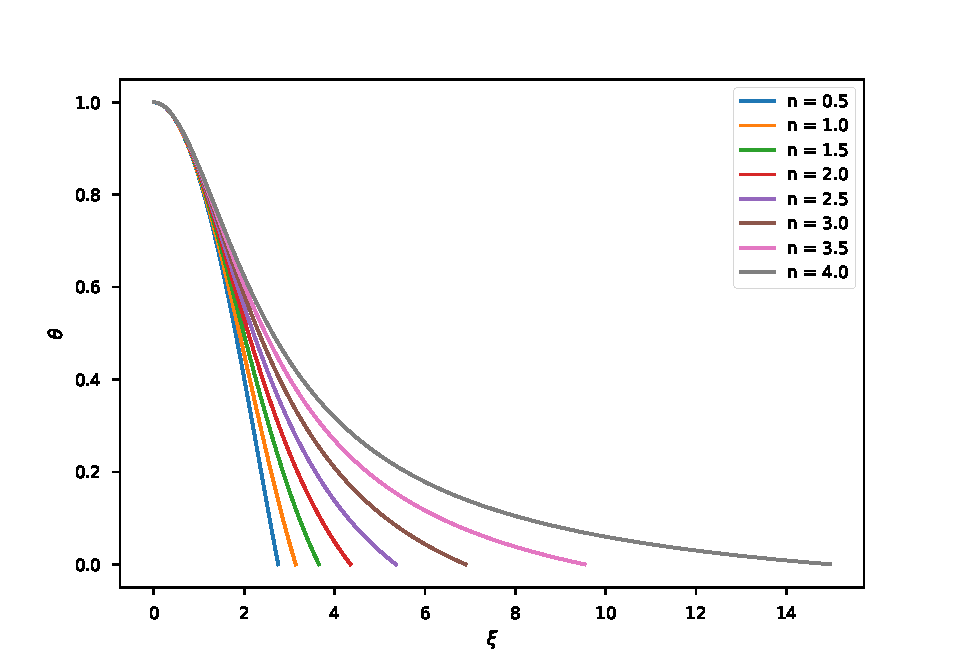
\includegraphics[width=\linewidth]{../figures/poly.pdf}
  \caption{Polytropic curves for varying index $n$}
  \label{fig:poly_ex}
\end{figure}

\subsection{Initial conditions and integration of first step}

Special attention is given to the first integration step, as we wish to avoid
the division by zero on $\xi = 0$.\footnote{We do this to avoid computational
  trouble. The singularity is otherwise removable.} We then start on an
arbitrarily small step $\delta \xi$ where we have relations 

\begin{equation}
  \label{eq:initial_cond_1}
  \theta(\delta \xi) = 1 - \frac{(\delta \xi)^2}{2} + \mathcal{O}\left((\delta \xi)^4\right)
\end{equation}
\begin{equation}
  \label{eq:initial_cond_2}
  \dot{\theta}(\delta \xi) = -\delta \xi + \mathcal{O}\left( (\delta \xi)^3 \right)
\end{equation}

\subsection{Shooting method for polytropic index determination}

If an observed value for luminosity is given one may use a shooting method to
determine a value of $n$ for which the luminosity at $\xi_s$ fits observed data.
Once again using a successive bisection method, finding the root of the scalar
function in equation \ref{eq:get_n} determined the polytropic index.

\begin{equation}
  \label{eq:get_n}
  y(n) = 1 - \frac{L_r(\xi_s)}{L}
\end{equation}

In the above prescription we did not need to explicitly know the value of $K$
(from equation \ref{eq:poly_relation}). The implications of this, along with
alternative cases, will be discussed in section \ref{sec:alternative_methods}.

\section{Sun - Example and code verification}
\label{sec:code_verification}

Firstly we take advantage of well know data for the Sun to verify the fidelity of the aforementioned method.

Our algorithm gives polytropic index $n = 3.197$ and normalized parameter
curves $(P, \rho, T)$ as seen in figure \ref{fig:sun_params}. As for emissivity,
we have the expected behavior of $\epsilon_{cno}$ dominance, and the
luminosity curve (with respect to relative mass) (figures
\ref{fig:sun_emissivity} and \ref{fig:sun_luminosity}).

\begin{figure}
  \centering
  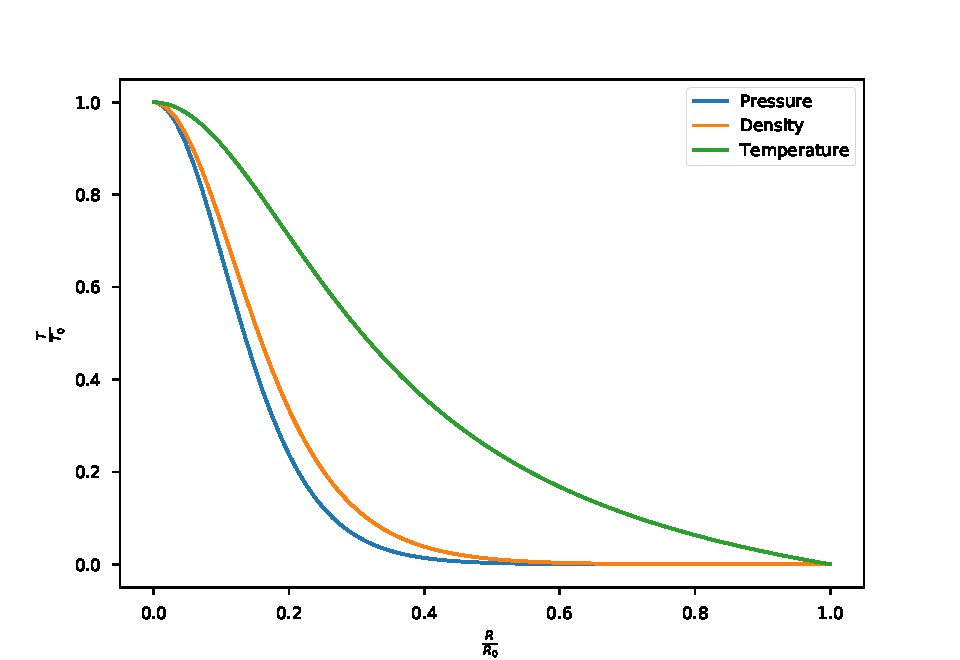
\includegraphics[width=\linewidth]{../figures/parameters_sun.pdf}
  \caption{Sun - Normalized parameters}
  \label{fig:sun_params}
\end{figure}
\begin{figure}
  \centering
  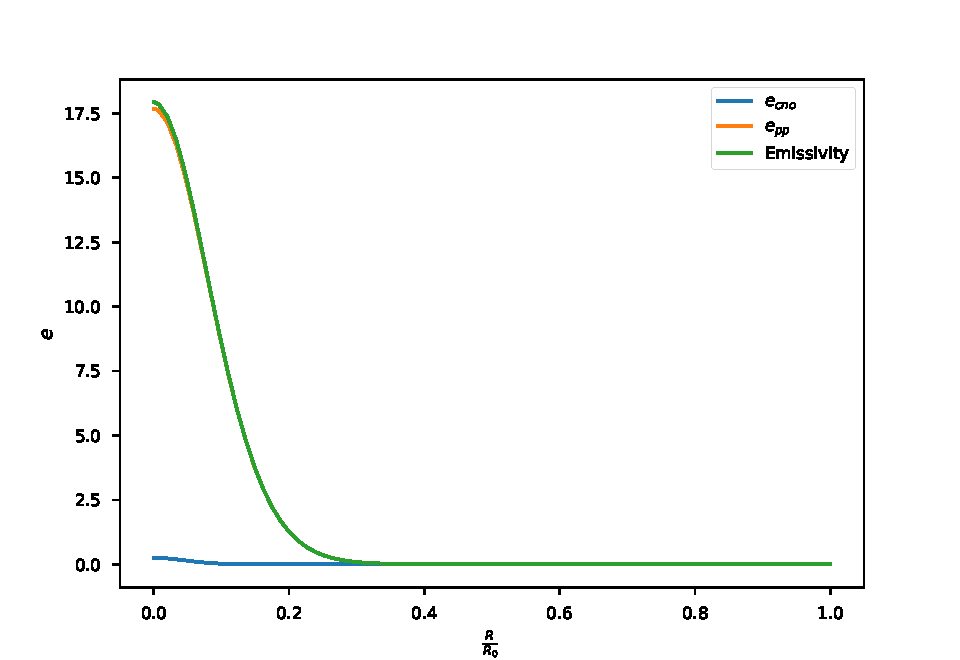
\includegraphics[width=\linewidth]{../figures/emissivity_sun.pdf}
  \caption{Sun - Emissivity}
  \label{fig:sun_emissivity}
\end{figure}
\begin{figure}
  \centering
  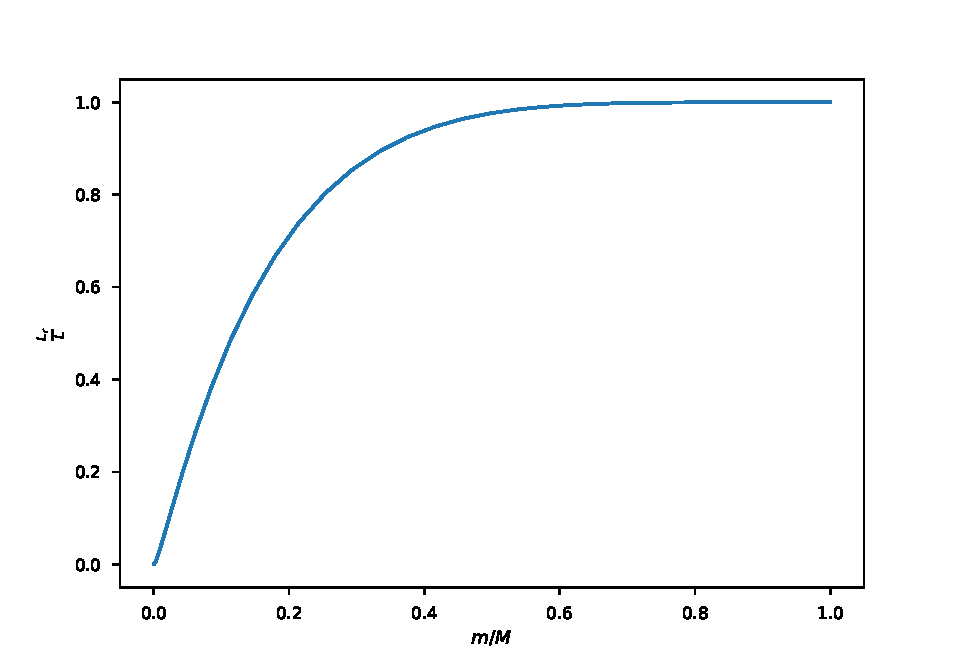
\includegraphics[width=\linewidth]{../figures/L_vs_M_sun.pdf}
  \caption{Sun - Luminosity}
  \label{fig:sun_luminosity}
\end{figure}

One may also calculate the energy of the polytrope and compare with the expected
analytical value, giving a measurement of the error of $n$. We use relation
\ref{eq:grav_test}, obtained utilizing equations \ref{eq:grav_analytical_energy}
and \ref{eq:grav_poly_energy}, as found in \cite{monteiro_sebenta_2019}, getting
$\delta n \approx 7 \times 10^{-7}$.

\begin{equation}
  \label{eq:grav_analytical_energy}
  V = \frac{3}{5-n} \frac{G M^{2}}{R}
\end{equation}

\begin{equation}
  \label{eq:grav_poly_energy}
  V = \frac{G M^{2}}{R} \frac{1}{\xi_{s}^{3} \theta_{s}^{\prime 2}} \int_{0}^{\xi_{s}} \xi^{3} \theta^{n} \dot{\theta} \mathrm{d} \xi
\end{equation}

\begin{equation}
  \label{eq:grav_test}
  \delta n = 3 \xi_{S}^{3} \theta_{S}^{\prime 2} \frac{1}{\int_{0}^{\xi_{s}} \xi^{3} \theta^{n} \dot{\theta} \mathrm{d} \xi} + 5 - n
\end{equation}

As will be discussed in section \ref{sec:applications}, this error is smaller
than the uncertainty (dependent on the uncertainty of observed data), so we are
reassured our method is appropriate, for the precision
required for our application is achieved.

\section{Applications - The $\alpha$ Centauri AB binary}
\label{sec:applications}

In this section we use observed data from \cite{bruntt_accurate_2010} (table \ref{tab:data}) to
estimate the polytropic index of $\alpha$ Centauri A and B. Uncertainty is
estimated by repeated sampling over normally distributed parameters of mass,
radius and luminosity in accordance to experimental uncertainty.

\begin{table}
  \centering
  \begin{tabular}{c  c  c}
    \toprule
    Parameter & $\alpha$ Centauri A & $\alpha$ Centauri B \\ \midrule
    Mass (M_\odot) & 1.105 \pm 0.007 & 0.934 \pm 0.006 \\
    Radius (R_\odot) & 1.225 \pm 0.004 & 0.864 \pm 0.005 \\
    Luminosity (L_\odot) & 1.47 \pm 0.05 & 0.47 \pm 0.02 \\
    Metallicity \footnote{No uncertainty is given for this parameter.} & 0.22 & 0.30 \\ \bottomrule
  \end{tabular}
  \caption{Observational data}
  \label{tab:data}
\end{table}

Calculated polytropic indices of both stars can be found in table \ref{tab:indices} and
parameter curves in figures \ref{fig:temperatures} to \ref{fig:luminosities}.

\begin{table}
  \centering
  \begin{tabular}{c  c}
    \toprule
    Star & Polytropic Index \\ \midrule
    Sun  & 3.197 \\
    $\alpha$ Centauri A & 3.472 \pm 0.005 \\
    $\alpha$ Centauri B & 2.87 \pm 0.02
  \end{tabular}
  \caption{Polytropic indices}
  \label{tab:indices}
\end{table}

\begin{figure}
  \centering
  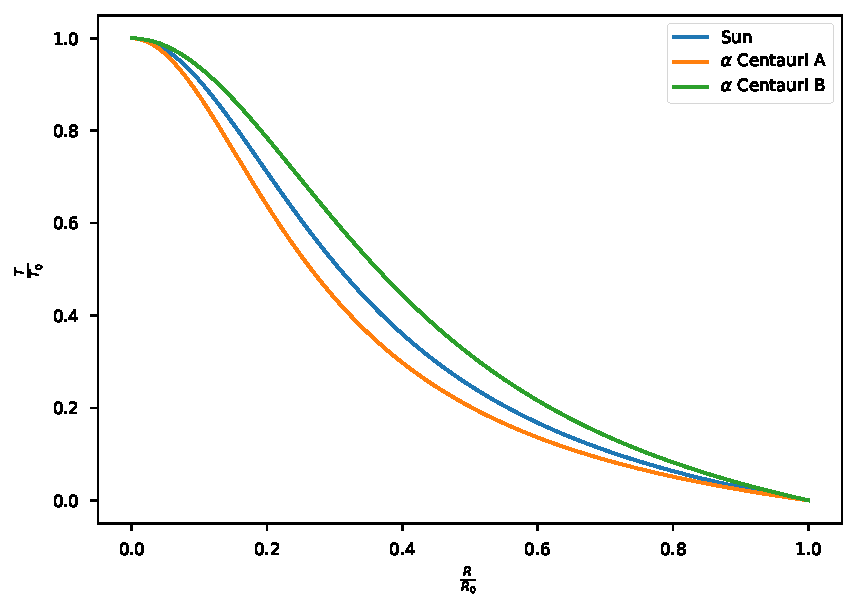
\includegraphics[width=\linewidth]{../figures/temperatures.pdf}
  \caption{Temperatures ($\alpha$ Centauri A, B and Sun)}
  \label{fig:temperatures}
\end{figure}
\begin{figure}
  \centering
  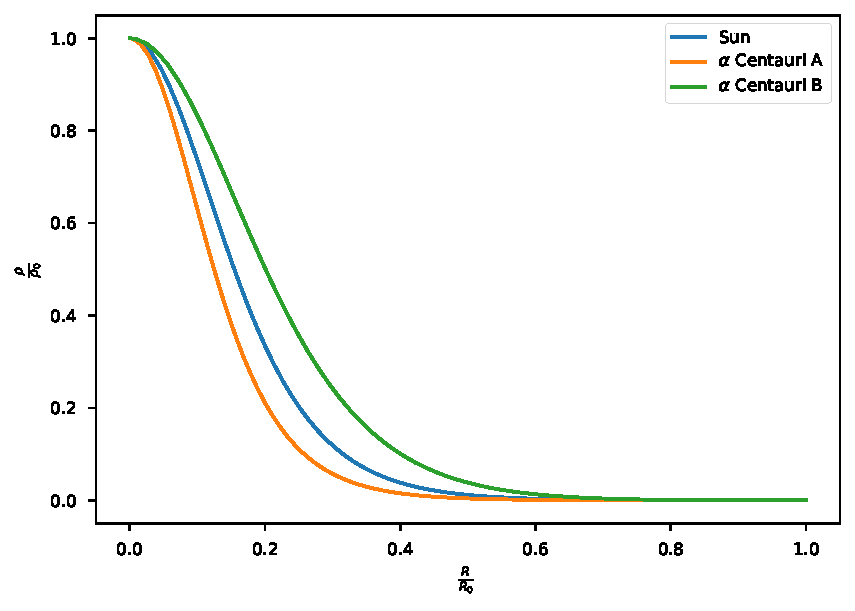
\includegraphics[width=\linewidth]{../figures/densities.pdf}
  \caption{Densities ($\alpha$ Centauri A, B and Sun)}
  \label{fig:densities}
\end{figure}
\begin{figure}
  \centering
  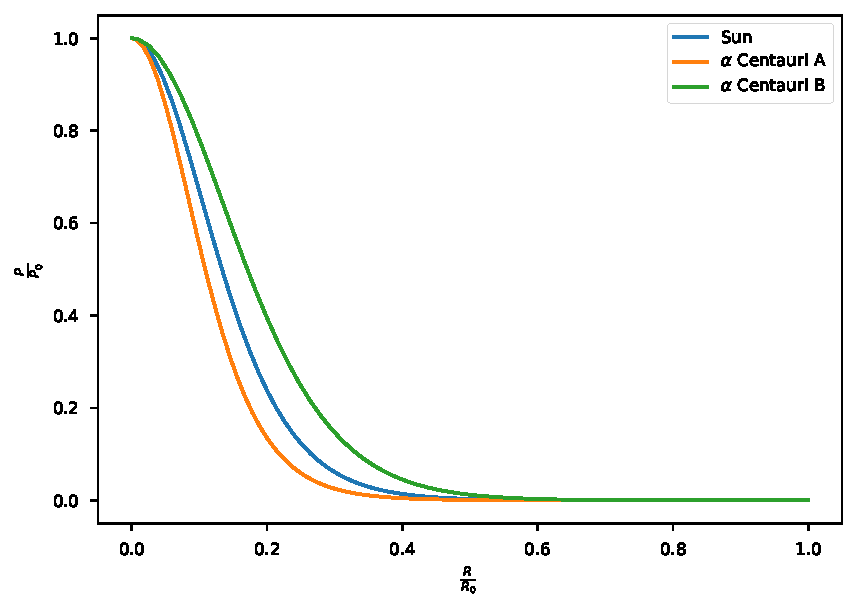
\includegraphics[width=\linewidth]{../figures/pressures.pdf}
  \caption{Pressures ($\alpha$ Centauri A, B and Sun)}
  \label{fig:pressures}
\end{figure}
\begin{figure}
  \centering
  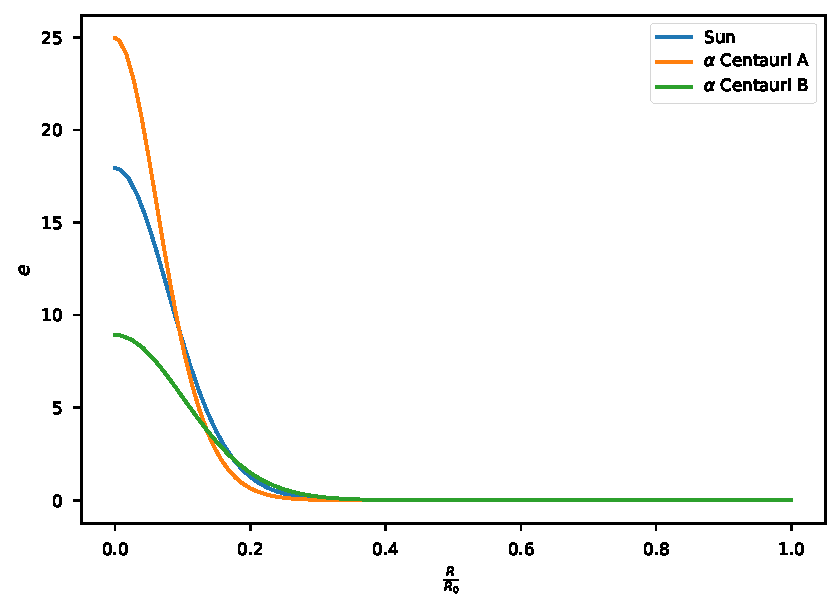
\includegraphics[width=\linewidth]{../figures/emissivities.pdf}
  \caption{Total emissivities ($\alpha$ Centauri A, B and Sun)}
  \label{fig:emissivities}
\end{figure}
\begin{figure}
  \centering
  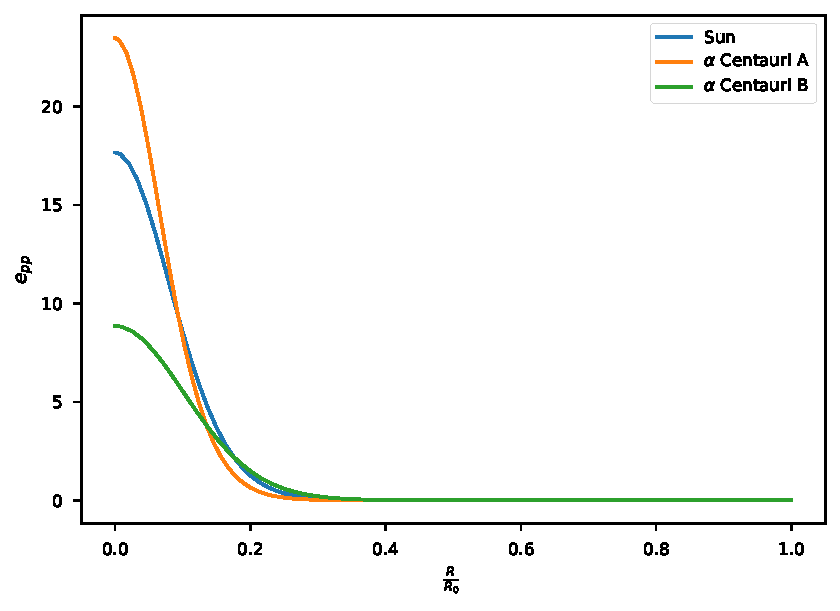
\includegraphics[width=\linewidth]{../figures/emissivities_pp.pdf}
  \caption{PP Emissivities ($\alpha$ Centauri A, B and Sun)}
  \label{fig:emissivities_pp}
\end{figure}
\begin{figure}
  \centering
  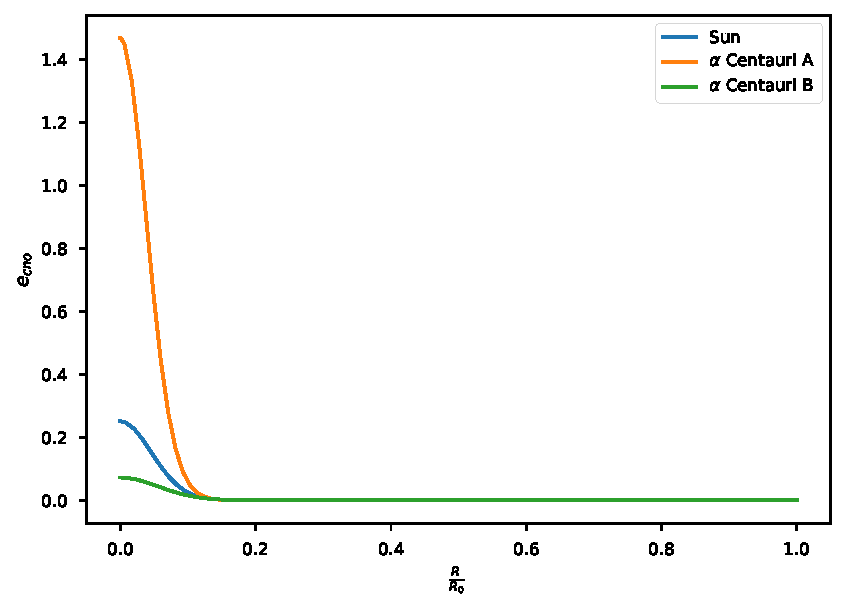
\includegraphics[width=\linewidth]{../figures/emissivities_cno.pdf}
  \caption{CNO emissivities ($\alpha$ Centauri A, B and Sun)}
  \label{fig:emissivities_cno}
\end{figure}
\begin{figure}
  \centering
  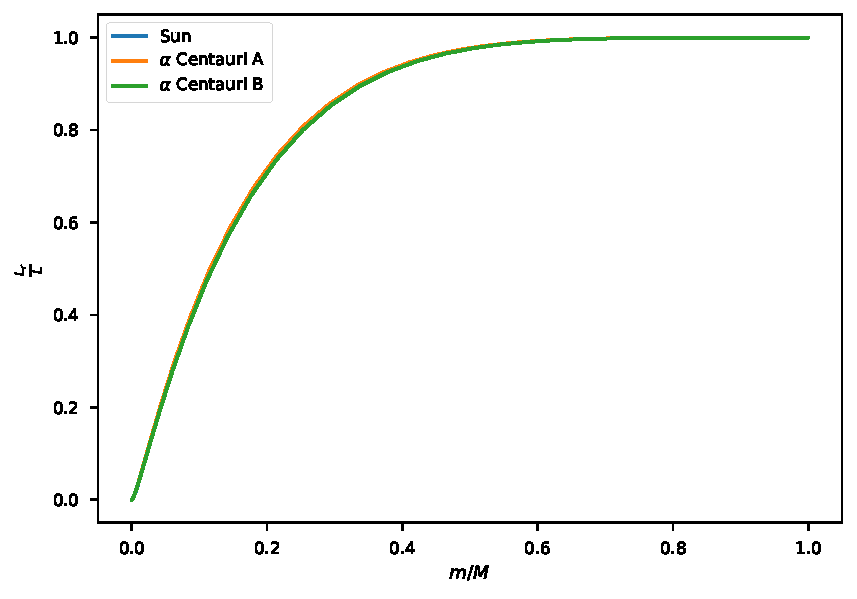
\includegraphics[width=\linewidth]{../figures/luminosities.pdf}
  \caption{Luminosities ($\alpha$ Centauri A, B and Sun)}
  \label{fig:luminosities}
\end{figure}

We see that to a higher polytropic index correspond curves of higher
relative temperature, pressure and density (figures \ref{fig:temperatures},
\ref{fig:densities} and \ref{fig:pressures}).

Another relevant trend is the significant increase of CNO emissivity with higher
$n$. Additionally, the slope of PP emissivity is proportional to the polytropic
index, seeing a more rapidly decreasing (though more intensive) curve for more
massive stars.

This is as expected, seeing as fusion of heavier elements (required for the CNO
cycle)  is more prevalent in condition of higher pressure and temperature. The higher slope
in more massive stars corresponds to the proportionally smaller nuclei where
radiative processes take place.
None of the stars analyses are sufficiently massive to see CNO cycle dominated emissivity.

When it comes to luminosity curves, a similar can be seen behavior from all parts, even
though absolute luminosity suffers significant variance.

Monte Carlo methods used for estimating uncertainty sampling $N = 10000$
iterations of simulated parameters within the experimental uncertainty. The
resulting index distribution can be inspected in figures \ref{fig:mc_alpha_a}
and \ref{fig:mc_alpha_b} for $\alpha$ Centauri A and B, respectively.

One may notice that these distributions are not symmetrical. This means only
that the expressions through which our error is propagated have non-linear
effects on said values, resulting in possibly asymmetrical distributions.

In rigor, one would give generally different uncertainty values corresponding for each side of
the distribution. On our case, however, we choose to give a more conservative
value, for reasons discussed in section \ref{sec:improvs}.

\begin{figure}
  \centering
  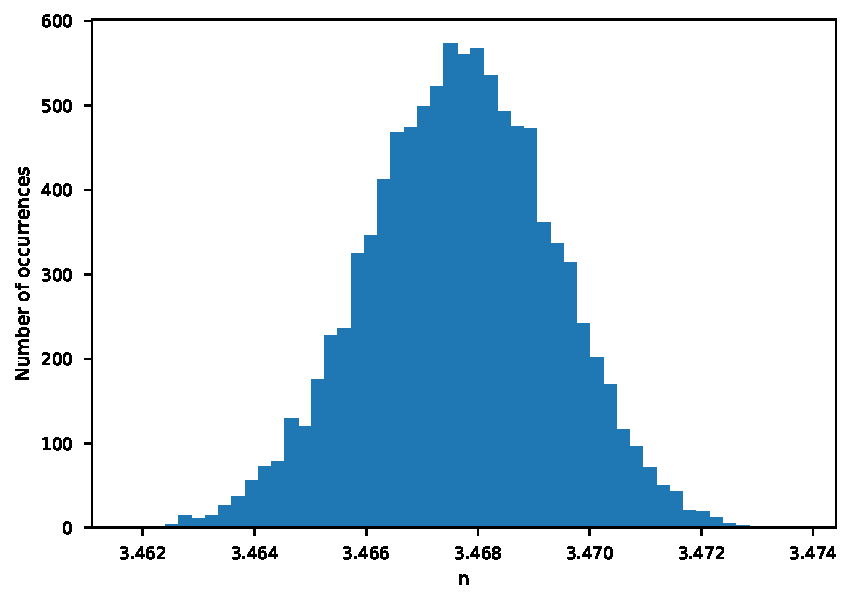
\includegraphics[width=\linewidth]{../figures/alpha_a_10k.pdf}
  \caption{$\alpha$ Centauri A - Monte Carlo index distribution}
  \label{fig:mc_alpha_a}
\end{figure}
\begin{figure}
  \centering
  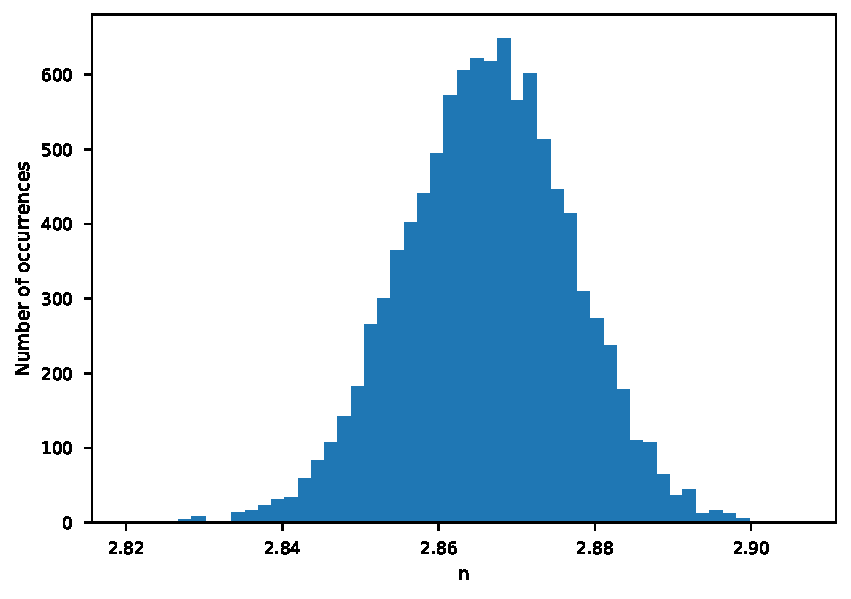
\includegraphics[width=\linewidth]{../figures/alpha_b_10k.pdf}
  \caption{$\alpha$ Centauri B - Monte Carlo index distribution}
  \label{fig:mc_alpha_b}
\end{figure}


\section{Valid regime and alternative methods}
\label{sec:alternative_methods}

\subsection{Alternative systems}

As referenced in section \ref{sec:method}, the way one formulates the problem
may have consequences on the choice of adequate boundary conditions, if any are needed.

A solution of equation \ref{eq:lane_emden} sets a value for $\xi_s$. A choice of
$M$ and $R$ provides a conversion factor to physical quantities (pressure,
density, temperature). This factors determine the value of $K$. For some
systems, however, like neutron stars, the polytropic relation is given by
physical considerations. This automatically sets a relation between the radius
and mass of the object, allowing us to construct the whole model from scarcer
data.

\subsection{Valid regime}
\label{sec:regime}

Even though equation \ref{eq:lane_emden} is general, given the assumptions
employed to construct our model, it may only be applied only in a given regime.
This enforces condition such as:
\begin{itemize}
\item electromagnetic forces can be ignored
\item system is fully characterized by a single polytropic index
\item system is in equilibrium
\end{itemize}
If using the shooting method, the star need be from the main
sequence, due to the assumptions made of the radiative processes leading to
the luminosity calculation.

\section{Model pathologies and possible improvements}
\label{sec:improvs}

The main pathology of our method lies in the assumption that the system is
described by a single polytropic condition. This assumption ignores, for
example, the fact that there might be an atmosphere affecting our calculation.

Multilayered systems could easily be included in our model (and even code, given
the modular nature of it). One would need only iteratively set boundary
conditions for each layer based on previous integration results.

This still does now allow for a full simulation of stellar structure, as a
fitting model of the atmosphere would need to be included, automatically setting
a boundary condition for the limiting density of our polytrope, $\theta_s$,
until which our algorithm would proceed in just the same way.

One could also include electromagnetic interactions, by using equations such as
found in \cite{takisa_charged_2013}.

A more significant improvement would be to include time dependence, permitting
the study of evolution. This, however, would require the time integration of
all four state equations, now out of equilibrium. This approach is much more
computationally intensive, but employed in super computers, using methods for
hydrodynamic equations such as found in \cite{kifonidis_multigrid_2012}.

\section{Conclusion}

\begin{itemize}
\item The polytropic model of stellar interiors was developed and the condition
  of its applications discussed.
\item An efficient numerical method for solving the Lane-Emden equation was implemented.
\item An algorithm for determining polytropic indices of main sequence stars
  from observed data (mass, radius, luminosity and chemical abundances) was presented.
\item This algorithm was applied to the study of the $\alpha$ Centauri AB
  binary. Stellar indices were determined and their influence on stellar
  structure analysed from constructed models.
\item Model limitations were studied and possible improvements discussed.
\end{itemize}

\begin{acknowledgements}
  This work was done under the orientation of professor Mário João Monteiro in the
  context of the curricular unit of Computational Astronomy.
\end{acknowledgements}

\bibliographystyle{aa}
\bibliography{poly}

\end{document}